\documentclass[11pt, a4paper]{article}

\usepackage{amsmath}
\usepackage[a4paper, margin=1in]{geometry}
\usepackage{amsfonts}
\usepackage{mathtools}

% to insert images
\usepackage{graphicx}
\graphicspath{ {./images/} {../images/}}

% \usepackage{hyperref}
% \hypersetup{
    % colorlinks=true, % make the links colored
    % linkcolor=blue, % color TOC links in blue
    % urlcolor=red, % color URLs in red
    % linktoc=all % 'all' will create links for everything in the TOC
% }

\setlength{\parindent}{0em}

% \DeclareMathOperator*{\minimize}{minimize}

\begin{document}
    %%%%%%%%%%%%%%%%%%%%%%%%%%%%%%%%%%%%%%%%%%%%%%%%%%%%%%%%%%%%%%%%%%%%%%%%%%%%%%%
    \section{Support Vector Machines}
    Maximal margin classifier is the first idea for the development towards SVMs. Maximal margin classifier utilizes hyperplanes and requires that the data is linearly separable. The extension of this is Support Vector Classifier that can be applied to an even broader class of problems. SVMs are a further extension of SVCs to account for non linear separation boundaries.
    

    %%%%%%%%%%%%%%%%%%%%%%%%%%%%%%%%%%%%%%%%%%%%%%%%%%%%%%%%
    \subsection{Maximal Margin Classifier}
    Maimum Margin Classifier uses hyper planes to find a separable boundary between the data points. Note that a hyperplane is simply a vector supspace of one less dimension. In 2 and 3 dimensions, hyperplanes are a line and a plane respectively. The general definition is
    \begin{align*}
        \beta_{0} + \beta_{1}X_{1} + \cdots + \beta_{p}X_{p} = 0
    \end{align*}
    Any point $X = (X_{1}, X_{2}, \ldots, X_{p})^{T}$ which lies on the plane will satisfy the above equation. Points satisfying the inequality $> 0$ will lie on one side and the ones satisfying $< 0$ will lie on the other side. Thus the hyperplane divides the whole $p$ dimensional space into two halves.\newline


    %%%%%%%%%%%%%%%%%%%%%%%%%%%%%%%%%%%
    \subsubsection{Classification}
    Suppose we have a set of data points with $p$ predictors and they belong to two classes given by $y_{i} = \{-1 , 1\{$. Suppose the points are perfectly separable through a hyperplane. Then the following hold
    \begin{align*}
        \beta_{0} + \beta_{1}x_{i1} + \cdots + \beta_{p}x_{ip} > 0 \text{ when } y_{i} = -1\\
        \beta_{0} + \beta_{1}x_{i1} + \cdots + \beta_{p}x_{ip} < 0 \text{ when } y_{i} = 1
    \end{align*}
    or, we can rewrite the above equation as
    \begin{align*}
        y_{i}(\beta_{0} + \beta_{1}x_{i1} + \cdots + \beta_{p}x_{ip}) > 0
    \end{align*}

    Thus classification can be made into the positive or negative class simply based on the sign of the quantity $\beta_{0} + \beta_{1}x_{i1} + \cdots + \beta_{p}x_{ip}$. The further a point is, the more confident we will be in the classification.\newline

    Note that there can be infinite such hyperplanes that perfectly separate data where each can be obtained by slightly perturbing the given plane. Define margin as the perpendicular distance from all observations in a given class. Then a minimum margin will be the one with the smallest perpendicular distance for all the points. This plane can be obtained for both the classes independently. The Maximal Margin Classifier should lie in the exact centre of two such planes.\newline

    \begin{figure}[h]
    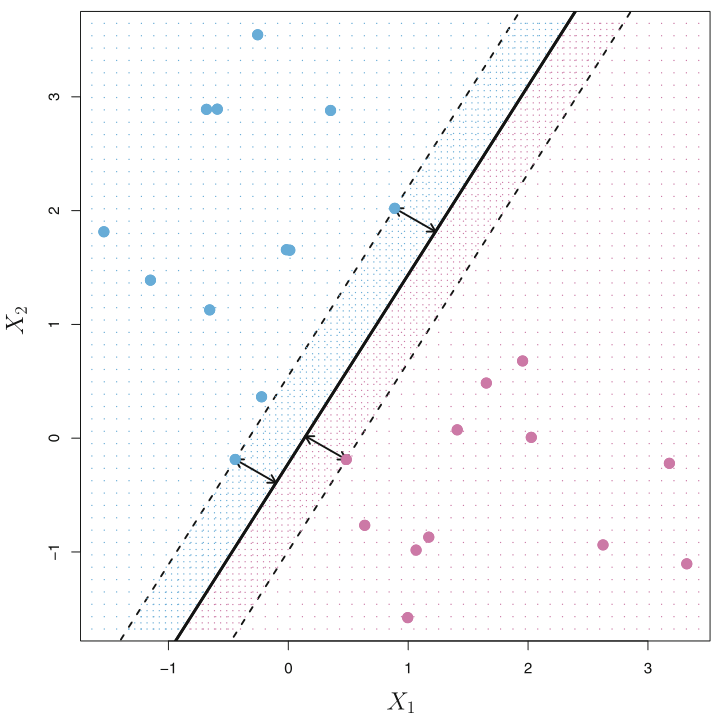
\includegraphics[scale=0.6]{mmc}
    \centering
    \caption{The Maximal Maargin Classifier with the Support Vectors}
    \label{fig:mmc} %\ref{fig:mmc}
    \end{figure}

    Note that the location of the maximal margin is determined only by the points closest to the boundary. If a point farther away would slightly move, the boundary would still be the same. Whereas if the point closer to the boundary would shift, the boundary itself would change as can be seen in figure \ref{fig:mmc}. These set of observations are know as \textbf{support vectors}.

    
    %%%%%%%%%%%%%%%%%%%%%%%%%%%%%%%%%%%
    \subsubsection{Algorithm}
    Finding the boundary is same as solving for the following optimization problem
    \begin{align*}
        \maximize_{\beta_{0},\ldots,\beta_{p}, M} M\\
        \text{subject to } \sum_{i=1}^{p} \beta_{i}^{2} = 1,\\
        \text{and } y_{i}(\beta_{0} + \beta_{1}x_{i1} + \cdots + \beta_{p}x_{ip}) \geq M \forall i = 1, 2, \ldots, n
    \end{align*}

    

\end{document}